\section{Introducción}

Queremos resolver el problema de los rankings de las páginas web, de manera que una búsqueda  sea más eficiente y a la vez que devuelva mejores resultados según algun criterio. 
Vamos a utilizar dos métodos para este propósito, cada uno de ellos tiene un criterio diferente para ordenar las páginas. \\

El primero se denomina $PageRank$. Es la primera versión del algoritmo que usó Google para posicionarse por encima de los otros buscadores en sus inicios. Usa propiedades de álgebra lineal y de matrices que vamos a enunciar en el trabajo y explicar en la medida que se necesite.\\

El segundo se denomina $IN-DEG$ y es mas sencillo, ya que sólo utiliza la cantidad de links entrantes de las páginas para definir el ranking.\\

El algoritmo de $PageRank$ es más complejo: Le asigna a cada página un puntaje que depende no solamente de la cantidad de links entrantes, sino de la importancia que tiene cada link, que depende del puntaje de la página de origen y de los links salientes de ella. Otro factor que afecta el ranking es la probabilidad de que el navegante salte a una página sin usar link. \\

De esta manera se evita que una página que es apuntada por muchas otras poco importantes, tenga mayor puntaje que otra que tiene menos links entrantes, pero que es apuntada por páginas más importantes. Este es un caso en que el algoritmo de $IN-DEG$ no da buenos resultados pero el $PageRank$ si.
%Veamos un ejemplo de esto, y los resultados de ambos algoritmos:\\


%Imagen de grafo de paginas 1
\begin{wrapfigure}{r}{0.6\textwidth}
  \vspace{-20pt}
  \begin{center}
    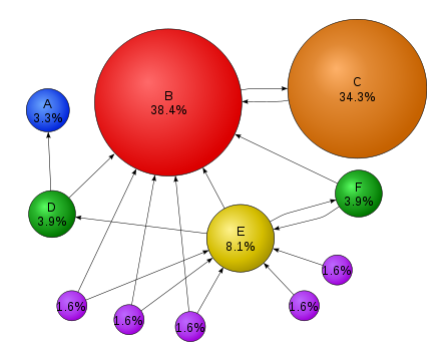
\includegraphics[scale= 0.6]{imagenes/ejemplo-grafo-1.png}
  \end{center}
  \vspace{-20pt}
   \caption[Caption for LOF]{El algebra lineal detrás de los buscadores de internet. Carlos D'Andrea.\footnotemark}
  \vspace{-10pt}
  \label{fig:img1}
\end{wrapfigure}



\footnotetext{Lectura: https://atlas.mat.ub.edu/personals/dandrea/2012_09_25_escrito_google.pdf.}

En el grafo de la figura 1, los nodos son páginas web y los ejes son los links. Los porcentajes muestran el orden en el ranking según el algoritmo de $PageRank$. La primera página es la B, luego la C, etc.\\

 Si aplicaramos el algoritmo de $IN-DEG$, la primera página tambien resultaría ser la B, pero la segunda la E. Y la C, que tiene un link entrante de la página que parece ser más importante (B), estaría en último lugar. En este ejemplo podemos ver la diferencia de los criterios de importancia de las páginas para ambos algoritmos.\\

Para este trabajo implementamos ambos algoritmos y analizamos los resultados obtenidos en diferentes escenarios.\\

También realizamos mejoras para el tiempo de ejecución y el espacio usado por el algoritmo de $PageRank$. Una forma de lograr esto es utilizar estructuras de datos que aprovechen ciertas condiciones que suelen darse en la realidad.\\

 Las optimizaciones que se hacen para reducir el tiempo y espacio de este algoritmo son importantes, porque es realidad es usado para procesar muy grandes cantidades de información y generar rankings de millones de páginas web. Haremos entonces un análisis temporal y espacial.\\

Por otro lado, hicimos una leve modificación al algoritmo de $PageRank$, para determinar rankings de equipos en una liga deportiva con un algoritmo que llamaremos $GeM$. \\

En $PageRank$ se representa a las páginas web como los nodos de un grafo en el que los ejes son los links. De la misma manera se puede representar a los equipos de una liga como los nodos y los resultados de los partidos como los ejes con un cierto peso, para determinar un ranking.\\

Como los grafos de las ligas no son tan grandes como los de las webs, no nos interesa analizar los aspectos mas computacionales del algoritmo, como tiempo y memoria. Vamos a analizar los diferentes resultados que obtuvimos con este algoritmo para un torneo de fútbol que ya terminó, y vamos a comparar los resultados obtenidos con $GeM$, un método propuesto por nosotros y el método estándar.\\


% imagen grafo4equipos
\begin{wrapfigure}{r}{0.5\textwidth}
  \vspace{-20pt}
  \begin{center}
    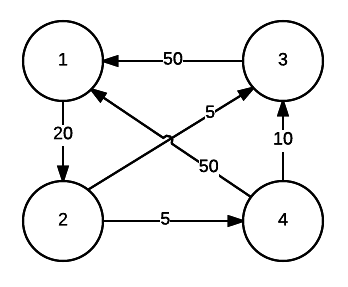
\includegraphics[scale= 0.8]{imagenes/grafo4equipos.png}
  \end{center}
  \vspace{-20pt}
  \caption{Mensaje a completar.}
  \vspace{-10pt}
  \label{fig:img2}
\end{wrapfigure}


El grafo de la figura 2 representa los partidos de una liga de algún deporte. Son 4 equipos (los nodos) y todos juegan contra los otros 3. Las aristas son la diferencia de puntos total de todos los partidos jugados entre los 2 equipos. Los nodos de llegada de las aristas son los equipos ganadores, es decir, que tienen una diferencia a favor.\\

Una alternativa para generar el ranking sería ordenarlos por cantidad de partidos ganados, y en caso de empate ordenarlos por puntos a favor. El ranking dejaría en primer lugar al equipo 1, en segundo lugar al equipo 3, en tercer lugar al equipo 2 y el último lugar el 4.\\

En cambio si usaramos el algoritmo de $PageRank$ para obtener el ranking, quedaría el equipo 1 en primer lugar también, pero en segundo lugar el equipo 2 y en tercero el 3. Esto es porque también importa a quien le ganó cada equipo, y el equipo 2 le ganó al 1 que tiene más partidos ganados y muchos puntos a favor. Con este algoritmo entonces podemos generar rankings que dependan de más variables.\\






